%%%%%%%%%%%%%%%%%%%%%%%%%%%%%%%%%%%%%%%%%%%%%%%%%%%%%%
%% Technische Universit�t M�nchen
%% Lehrstuhl f�r Datenverarbeitung
%% Latex-Template
%% Kontakt: 
%% Stand: 16.10.2018
%%%%%%%%%%%%%%%%%%%%%%%%%%%%%%%%%%%%%%%%%%%%%%%%%%%%%%

%% *** Dokumentinformationen ***
\newcommand{\AutorVorname}{Tobias}									% Vorname des Verfassers
\newcommand{\AutorNachname}{Hofmann}								% Nachname des Verfassers
\newcommand{\AutorEmail}{tobias.th.hofmann@tum.de}		% Emailadresse des Verfassers

\newcommand{\Semester}{Sommersemester 2021}			% Aktuelles Semester: Sommersemester JJJJ bzw. Wintersemester JJJJ
\newcommand{\SemesterShort}{SS 2021}					  	% Aktuelles Semester: SS JJJJ bzw. WS JJJJ
\newcommand{\DatumAbgabe}{12.07.2021}								
\newcommand{\Thema}{Monty Matlab: Group 5}					% Thema der Arbeit
\newcommand{\Keywords}{Schlagw�rter anstelle von Index Terms verwenden} % Schlagw�rter (maximal 5 St�ck, durch Kommata getrennt)

%% *** Dokumenteigenschaften ***
%%%%%%%%%%%%%%%%%%%%%%%%%%%%%%%%%%%%%%%%%%%%%%%%%%%%%%
%% Technische Universit�t M�nchen
%% Lehrstuhl f�r Elektrische Energiespeichertechnik
%% Latex-Vorlage f�r Short Paper/Hauptseminar
%% Kontakt: 
%% Stand: 10.05.2013
%%%%%%%%%%%%%%%%%%%%%%%%%%%%%%%%%%%%%%%%%%%%%%%%%%%%%%

%% *** IEEE (S) Dokumentklasse ***
\documentclass[10pt]{IEEEStran}


%% *** Schriften und Sprache ***
	\usepackage[latin1]{inputenc}		% Texcodierung
	\usepackage[T1]{fontenc}				% T1 Schriften
	\usepackage[english]{babel}			% deutsche Silbentrennung und Beschriftungen
	%\usepackage{mathptmx} 					% Times Schriftart
	%\usepackage[scaled]{helvet} 		% Helvetica Serifenfreie Schriftart
	%\usepackage{courier}
	\usepackage[babel,german=quotes]{csquotes} % Deutsche Anf�hrungszeichen mittels \enquote{}
	\usepackage{xspace}							% Intelligente Leerzeichen


%% *** Bilder und Geometrie ***
	\usepackage[pdftex]{graphicx}			% Grafiken einbinden
	
		\graphicspath{{IMG/}} 												% Pfad f�r Bilder angeben
		\DeclareGraphicsExtensions{.pdf,.jpeg,.png}		% Endungen die eingebunden werden
	\usepackage[caption=false,font=footnotesize]{subfig}	% Caption wird von IEEE �bernommen: http://www.ctan.org/tex-archive/macros/latex/contrib/subfig/
	\usepackage[a4paper,left=1.65cm,right=1.65cm,top=1.78cm,bottom=1.78cm,includeheadfoot]{geometry}
	%\usepackage{pdfpages}						% PDF Dateien einf�gen
	%\usepackage{color}								% Farben erm�glichen
	%\usepackage{capt-of}
	%\usepackage{setspace}	


%% *** Tabellen ***
	%\usepackage{longtable}						% Tabellen �ber mehrere Seiten
	\usepackage{array}								% erweitern Tabelleneigenschaften: http://www.ctan.org/tex-archive/macros/latex/required/tools/
	\usepackage{mdwtab}								% http://www.ctan.org/tex-archive/macros/latex/contrib/mdwtools/
	%\usepackage{booktabs}
	%\usepackage{tabularx}
	%\newcolumntype{C}{>{\centering\arraybackslash}X}


%% *** Mathe ***
	\usepackage[cmex10]{amsmath}
		\interdisplaylinepenalty=2500 	% Verhindert Seitenumbruch bei l�ngeren Formeln
	\usepackage{mdwmath}							% http://www.ctan.org/tex-archive/macros/latex/contrib/mdwtools/
	\usepackage{amsmath,amsfonts,amssymb}
	\usepackage[squaren,textstyle]{SIunits}
	%\usepackage{siunitx}  
	%\sisetup{locale = DE, per-mode=symbol,range-units=single} 
	\usepackage{icomma}

%Abk�rzungsverzeichnispakete
\usepackage[nolist]{acronym}
	
	
	
%% *** Algorithmen ***
	%\usepackage{algorithmic} 				% http://www.ctan.org/tex-archive/macros/latex/contrib/algorithmicx/
		%\floatname{algorithm}{Algorithmus}
		%\renewcommand{\algorithmicfor}{\textbf{F�r}}
		%\renewcommand{\algorithmicdo}{\textbf{:}}
		%\renewcommand{\algorithmicendfor}{}

	
%% *** Quellcode ***
	%\usepackage{listings}						% Direktes einbinden von Quellcode
	%\usepackage{verbatim}						% Quellcode anstatt Listings
	%\usepackage[numbered]{mcode}			% MatLab Code
	%\renewcommand{\lstlistingname}{Quellcode}


%% *** Einstellungen ***
	%\setcounter{secnumdepth}{4}				% Kapitelnummerierung mit x Ebenen
	%\setcounter{tocdepth}{4}					% Eintrag ins Inhaltsverzeichnis bis Ebene x
	%\definecolor{Gray}{gray}{0.4}
	%\onehalfspacing
		
	%\setlength{\parindent}{0mm}			% Erstzeileneinzug bei neuem Absatz
	%\setlength{\parskip}{8pt}				% Abstand zwischen Abs�tzen einstellen
	%\setcapindent{1em}								% Zeilenumbruch bei Bildbeschreibungen


%% *** Kopf- und Fusszeile ***
	%\usepackage{scrpage2}							% Seitenlayout KOMA-Script
	%\pagestyle{scrheadings}
	%
	%\automark[section]{chapter}
	%\setheadsepline{1.0pt}[\color{Gray}]
	%
	%\ihead{}
	%\chead{}
	%\ohead{\color{Gray}\textbf{\headmark}}

	
%% *** Nummerierung und Beschriftung ***
	%\addtokomafont{captionlabel}{\normalfont\bfseries}
	%\addtokomafont{caption}{\normalfont\bfseries}


%% *** Literatur ***
	%\usepackage{cite}								% http://www.ctan.org/tex-archive/macros/latex/contrib/cite/
	% cite.sty was written by Donald Arseneau
	% V1.6 and later of IEEEtran pre-defines the format of the cite.sty package
	% \cite{} output to follow that of IEEE. Loading the cite package will
	% result in citation numbers being automatically sorted and properly
	% "compressed/ranged". e.g., [1], [9], [2], [7], [5], [6] without using
	% cite.sty will become [1], [2], [5]--[7], [9] using cite.sty. cite.sty's
	% \cite will automatically add leading space, if needed. Use cite.sty's
	% noadjust option (cite.sty V3.8 and later) if you want to turn this off.
	% cite.sty is already installed on most LaTeX systems. Be sure and use
	% version 4.0 (2003-05-27) and later if using hyperref.sty. cite.sty does
	% not currently provide for hyperlinked citations.
	
	\usepackage[numbers]{natbib}
	
	% *** Chronologische Sortierung ***
	%\bibliographystyle{EES_DIN1505_UNSRT}
	
	% *** Alphabetische Sortierung ***
	%\bibliographystyle{EES_DIN1505_ABBRV}
	\bibliographystyle{EES_STANDARD}
	
	\renewcommand{\refname}{List of Bibliography}	% Literatur in Literaturverzeichnis umbenennen


%% *** PDF, URL und HYPERLINK Packete ***
%% *** MEISTENS ALS LETZES EINBINDEN! ***
	\usepackage{url}															% Einf�gen von URLs: \url{my_url_here}
	\usepackage{float}														% http://www.ctan.org/tex-archive/macros/latex/contrib/float
	\newcommand\MYhyperrefoptions{
		bookmarks					= true,
		bookmarksnumbered	= true,
		pdfpagemode				= {UseOutlines},
		plainpages				= false,
		pdfpagelabels			= true,
		colorlinks				= true,
		linkcolor					= {black},
		citecolor					=	{black},
		urlcolor					= {blue},
		bookmarksopen			= false
	}

	\ifCLASSINFOpdf
		\usepackage[\MYhyperrefoptions,pdftex]{hyperref}
	\else
		\usepackage[\MYhyperrefoptions,breaklinks=true,dvips]{hyperref}
		\usepackage{breakurl}
	\fi
	
	\hypersetup{
		pdftitle			= {Hauptseminar},
		pdfauthor			= {\AutorVorname \AutorNachname},
		pdfsubject		= {\Thema},
		pdfkeywords		= {\Keywords},
		pdfcreator		= {LaTeX},
		pdfproducer		= {LaTeX}
	}


\begin{document}
%%%%%%%%%%%%%%%%%%%%%%%%%%%%%%%%%%%%%%%%%%%%%%%%%%%%%%
%% Technische Universit�t M�nchen
%% Lehrstuhl f�r Elektrische Energiespeichertechnik
%% Latex-Vorlage f�r Short Paper/Hauptseminar
%% Kontakt: 
%% Stand: 10.05.2013
%%%%%%%%%%%%%%%%%%%%%%%%%%%%%%%%%%%%%%%%%%%%%%%%%%%%%%

\newcommand{\zb}{z.\,B.\xspace}		% um mit \zb z.B. einzugeben
\renewcommand{\figurename}{Fig.}	% Abb. statt Abbildung als Label
\renewcommand{\tablename}{Tab.}		% Tab. statt Tabelle als Label

%% *** Titel der Arbeit ***
\title{\Thema}

%% *** Autor und Betreuer ***
\author{Authors: \textit{Tobias~Hofmann},
				\textit{Tobias~Krug},
				\textit{Rayene~Messaoud},
				\textit{Alexander~Sch�lles}}% <-this % stops a space


%% *** Kopfzeile ***
\markboth{Lehrstuhl f�r Datenverarbeitung -- Monty Matlab \SemesterShort}{}
\maketitle

%% *** Abstract ***
\begin{abstract}
% very short motivation and problem overview
\ac{ML} is widely used in many human behavior classification applications. This work deals with binary classification of acceleration data, recorded with an IMU-sensor of any smartphone. We show how to exploit characteristics of normal and unnormal walking. Different approaches, feature selections and hyperparameters are discussed.
% Goals and topics of the work
In addition to the classification algorithm, we identify diverse data, preprocessing and a straightforward \ac{GUI} to guide the development as crucial elements to yield a high accuracy.
Additionally, different \ac{ML} techniques are evaluated and discussed. To determine the most accurate approach, a MATLAB implementation for training, testing and validation is carried out to determine the best performing model.
% Main Results
A stacked model of a \ac{SVM}, a \ac{RF} and three \ac{LSTM} networks yields the highest balanced accuracy with \unit{99.5196}{\%} on the test data. The \ac{SVM} and \ac{RF} use an amount of 102 features per acceleration dimension to learn the walking patterns. The three \ac{LSTM} networks operate with 36, 213 and 378 hidden units to track different dynamics of human gait.
\end{abstract}

%% *** Keywords & Acronym ***
%% *** Keywörter ***
\begin{IEEEkeywords}
%\Keywords
Classification, Gait Recognition, MATLAB, Neural Networks, Artificial Intelligence, Data Engineering
\end{IEEEkeywords}
%
% Abkürzungsverzeichnis
%\addcontentsline{toc}{section}{Abkürzungsverzeichnis}
%\section*{Abbreviations}
\begin{acronym}[Bash]
 \acro{SVM}{Support Vector Machine}
 \acro{RF}{Random Forest}
 \acro{GUI}{Graphical User Interface}
 \acro{ML}{Machine Learning}
 \acro{LSTM}{Long Short-Term Memory}
 \acro{NN}{Neural Network}
\end{acronym}


% *** Introduction ***
% Motivation and related works. 0.5 Page
%% *** 1. Kapitel ***
\section{Introduction}
% *** Motivation ***
% Which problem leaded to this work?
% In which research area? Which challenges can occur?
\IEEEPARstart{A}{nalysing} the walking behavior of a person is considered easy for the human eye. In contrast several challenges arise if a computer is tasked with this decision. Firstly, a feasible sensor, e.g. an IMU sensor in a smartphone, needs to be monitored. Secondly, preprocessing is needed before feeding any algorithm. At last, the computer requires the right algorithms and parameters to yield high accuracy - for training, testing and validation accuracy.\\
We present a \ac{ML} approach and a \ac{GUI} that allows preprocessing, training/testing and inspection of recorded gait data. The resulting model is able to distinguish between normal and unnormal gait.
% *** State of the Art *** -> cite related papers
IMU-based classification of human movement data is well discussed in literature. Most of the works use a \ac{ML} approach, like \ac{SVM}, \ac{RF} or Neural Networks to recognize diseases, e.g. Parkinson. In general very high accuracies can be reached \cite{Caramia2018, Ajani2019, Cuzzolin2017}.\\
% *** Goals of this work ***
This work aims to develop a combined \ac{ML} model to reach high accuracies for binary classification of acceleration time series data from recorded gaits.
% *** This Paper ***
% Which working steps are included and which are not?
This paper focuses on the algorithm itself and not on the preprocessing or the \ac{GUI}.
% Why and how is this work stand-alone?
In contrast to other works building on feature dependent algorithms alone, we employ a stack of \ac{SVM}, \ac{RF} and three \ac{LSTM} networks.
% *** Methodology and Workflow ***
% How should the goals of this work be reached?
To reach the goal of high testing and validation accuracy, optimal parameters for data split and hyperparameters of applied \ac{ML} algorithms need to be determined iteratively.
% How was proceeded?
The impact of said features, hyperparameters and their combination are evaluated and discussed.
% How is the work structured?
The paper presents the \ac{ML} approaches and the selected features. Further, the best combination of individual classifiers and their hyperparameters are outlined and results are discussed.


% *** Main Part ***
% Problem Overview, Implementation (flowchart). 1 Page
\section{Method and Discussion}
 The pipeline is depicted in \autoref{img:flwPipe}. It consists of a first stage, wherein the raw data is trimmed to remove irrelevant data at the start and end. The same stage automatically splits the data according to the selected training ratio of 70:30. From then on, one part of the data is used as training data to train the actual classifier ensemble depicted in \autoref{img:flwClass} and the other is used as test data to rate the trained models\footnote{Validation data and training/testing data were acquired by different people to support the calculation of reliable validation/generalization figures.}.

\begin{figure}[hbtp]
\centering
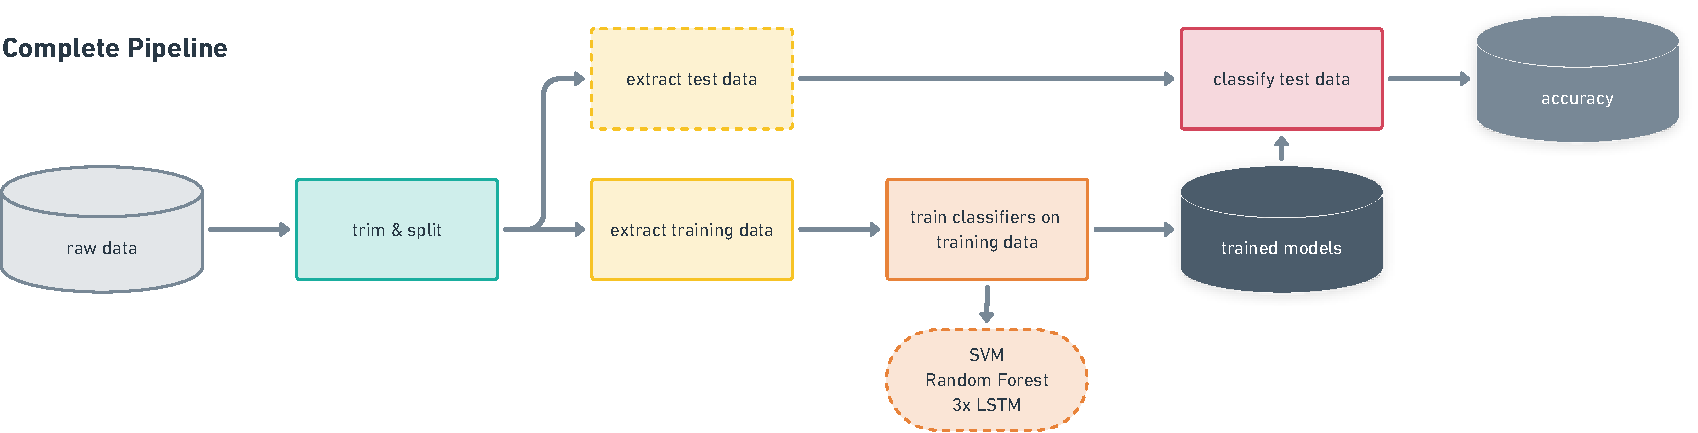
\includegraphics[width=\linewidth]{Flowchart-Pipeline.pdf}
\caption{Flowchart of the complete data processing pipeline}
  \label{img:flwPipe}
\end{figure}

The model itself consists of five classifiers, each with specific settings regarding whether to sort the axes by their mean to compensate for different orientations during data acquisition, which features to use, how many iterations to train and how many hidden units to configure in the \ac{LSTM} layer of the \acp{NN}. \autoref{img:flwClass} shows how the \ac{SVM} and \ac{RF} are feed with features, whereas the \acp{LSTM} are directly working on the time-series data. Depending on the settings, our proposed ensemble operates either in 1-stage or 2-stage stacking scenario. Our test yielded, that the 1-stage stack provides superior testing accuracy, while still working reasonably well on validation data.

\begin{figure}[hbtp]
\centering 
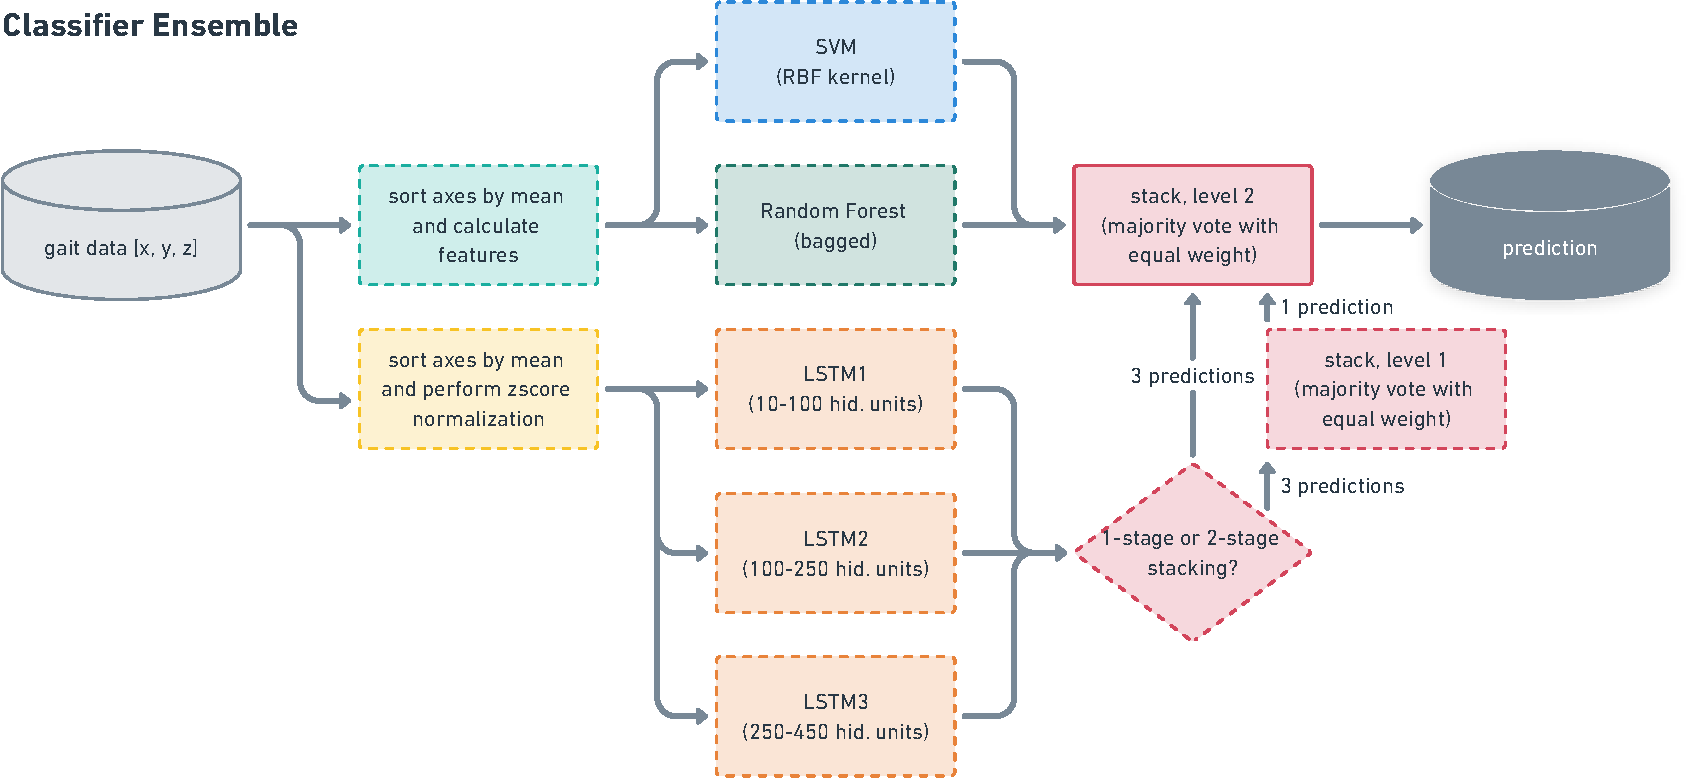
\includegraphics[width=.84\linewidth]{Flowchart-ClassifierEnsemble.pdf}
\caption{Flowchart of classifier ensemble architecture}
  \label{img:flwClass}
\end{figure}

% Optimization Process
The search for the optimal model was done in an iterative manner. The optimization target was chosen as the mean balanced accuracy of the model when applied on training, testing and validation data. In total eleven cycles with an amount of 234 models were trained and evaluated. The results of the 10th cycle are shown in table \ref{tbl:opt_process}. The goal was to determine the impact of nondeterminism introduced by MATLAB's LSTM training procedure by training 20 different models with the final settings. Table \ref{tbl:opt_process} summarizes the results of this cycle and shows a remarkable mean balanced accuracy on test data of almost \unit{99}{\%} for the final settings.
The entry point for this cycle was determined by choosing the most promising model from the previous 9 optimization cycles. There we applied a parameter sweep across all settings.
The final model has a unique combination of outstanding balanced accuracy on test data, good validation performance, fast classification (as \ac{SVM} and \ac{RF} operate with the same feature settings which allows a combined feature extraction), and short training time.
 
%% Tabelle einfügen
\begin{table}[h]
     \centering
     \caption{Statistics on the balanced accuracy of 20 trained models with final settings}
     \begin{tabular}[h]{p{2cm}||p{1cm}|p{1cm}|p{1cm}|p{1cm}}
     Metric & Max [\%]& Min [\%]& Mean [\%]& Std [\%] \\
     \hline
     mean of mean (train, test, val.) &$96.73$&$95.23$&$96.02$&$0.235$\\
     training &$100$&$99.92$&$99.96$&$0.030$\\
     testing &$99.52$&$97.85$&$98.82$&$0.408$\\
     validation &$90.71$&$86.72$&$89.29$&$0.927$  \\
     \end{tabular}
	\\
     \label{tbl:opt_process}
     % Verweis im Text mittels \ref{tbl:beispieltabelle}
   \end{table}

Subsequently, the model with the highest testing accuracy was chosen as it promises to perform well on data acquired by other people with similar movements while still supporting generalization as is indicated by its validation accuracy. The model reached a balanced accuracy on training data of \unit{99.9693}{\%}, on test data of \unit{99.5196}{\%} and on validation data of \unit{90.7076}{\%}.

 % Features + SVM + RF Classifier
The feature-based models \ac{SVM} and \ac{RF} are fed with feature vectors instead of the preprocessed data. Before assessing the features, the axes of acceleration data are sorted by mean value to tackle the problem of varying phone orientation during data recording. Besides basic statistical features like mean and variance, advanced features like the Shannon Entropy or the Wavelet Leader Estimation are evaluated and combined in a feature vector.

While the \ac{SVM} model trains with a maximum number of 200 iterations using randomsearch, the \ac{RF} classifier uses a bagging ensemble technique with 100 iterations.

Further the optimization process yielded the improvement by introducing multiple \ac{LSTM} networks in parallel - each adapting to different time horizons of human gait dynamics. Therefore three networks are placed in parallel with 36, 213 and 378 hidden units respectively. The training was done with a minibatch size of 20 and an epoch limit of 30. Similarly to the feature extraction, an axes-sorting algorithm was implemented and contributed to a higher accuracy.

Figure \ref{img:confmat} depicts the confusion matrix of the final model. The classification procedure runs almost instantaneously while maintaining the mentioned accuracy figures. This supports potential applications in real-time systems like gait classification in phones, smart-watches or similar.

\begin{figure}[hbtp]
\centering 
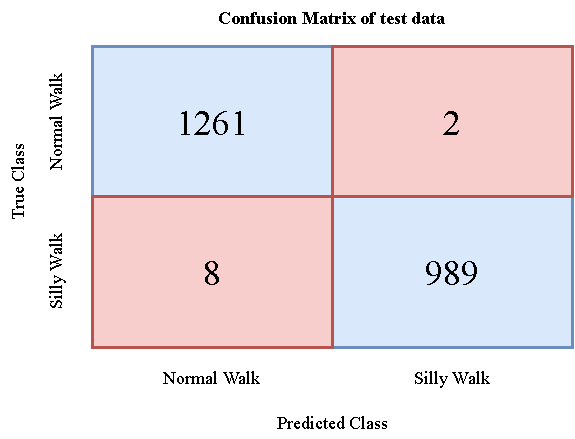
\includegraphics[width=.7\linewidth]{ConfusionMatrix.pdf}
\caption{Confusion Matrix of the final model on the test data}
  \label{img:confmat}
\end{figure}


 
 

% *** Conclusion ***
% Conclusion, Discussion and known issues. 0.5 Page
\section{Conclusion}
To conclude, we show a data-driven approach that was derived during an extensive optimization procedure. We yield a powerful model to classify acceleration data from human gait recorded with smartphones. The combination of \ac{LSTM} models, which work with time series data, and feature-based models, namely \ac{SVM} and \ac{RF}, achieves an accuracy of more than \unit{99}{\%}. Empirical research by the authors showed that 1-stage stacking is the optimal way to implement this combination, while 2-stage stacking pretends to perform better on generalization - indicated by the higher validation accuracy.

We estimate further potential by enhancing the axes-sorting algorithm. This could be done by coordinate transformation in case 6- or 9-axes IMU-sensor-data is available. This technique may improve performance and reduce the false positive rate. This would allow new applications e.g. to recognize Parkinson or other gait-affecting conditions.

%% *** Anhang (wenn benoetigt) ***
\appendices
%\addchap{Anhang}
\label{sec:Anhang}



\bibliography{Literatur}

%%%%%%%%%%%%%%%%%%%%%%%%%%%%%%%%%%%%%%%%%%%%%%%%%%%%%%%%%%%%%%%%%%%%%%%%%%%%%%%
\end{document}


